\section{Results}
\label{sec:results}

We organize the evidence around four questions. RQ1 asks whether a learned
policy changes the simple-policy frontier. RQ2 tests whether the decision
persists across question samples and retrieval environments. RQ3 compares the
information carried by four signal roles. RQ4 evaluates our optional
certificate.

\subsection{RQ1: Does learning change the frontier?}

\begin{figure}[t]
  \centering
  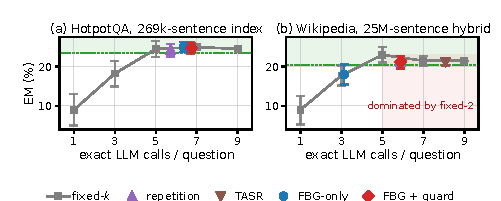
\includegraphics[width=\columnwidth]{figures/fig_frontier_main.pdf}
  \caption{Accuracy versus exact LLM calls in the primary HotpotQA and
  Wikipedia 25M cells. Shading marks the 1-EM admissible band and the fixed-2
  domination region.}
  \label{fig:frontier}
  \Description{Two scatter plots of exact-match accuracy against exact LLM
  calls per question for fixed budgets, answer repetition, TASR, and learned
  stopping policies. Vertical bars show paired 95 percent intervals against
  the full-budget policy. A green band spans accuracies within 1 exact-match
  point of the full budget. In the right panel a red block covers costs at or
  above the fixed-2 budget with accuracy at or below it.}
\end{figure}

\paragraph{Full-budget savings overstate adaptive value.}
On the nine-backbone HotpotQA panel with call accounting, FBG-only removes 27 to
57\% of searches relative to the full budget. Its paired EM differences range
from $-2.1$ to $+2.0$ points, and seven of nine intervals contain zero. The
stronger point-frontier comparison yields a different conclusion. Across the
core 26 cells, FBG-only is dominated in 10 cells, lies on the frontier
without improving $B^\star$ in 13, and improves $B^\star$ in 3. Guarded FBG is
dominated in 15 of 26 cells, is frontier-only in 6, and improves $B^\star$ in
5. Thus it fails to strictly improve the selected fixed budget in 21 of 26
cells. Table~\ref{tab:decision-matrix} reports the complete matrix. Its first
block contains 12 call-only cells, while the final block contains 14 fully
instrumented cells. In the table, C denotes exact LLM calls, $\Delta$ compares
a learned policy with the full budget, and Cat. gives its D, F, or I point
category. These categories prevent a cheap but inaccurate point from being
described as a tie. Cert. gives the SGR outcome. NA marks unavailable
raw features and `refuse' zero certificate coverage.

\begin{table*}[t]
\caption{Complete FBG point audit across 12 call-only and 14 fully instrumented
core cells.}
\label{tab:decision-matrix}
\scriptsize
\setlength{\tabcolsep}{2.6pt}
\rowcolors{3}{}{rowshade}
\begin{tabular}{l r r r r r l c r l c l}
\toprule
\hiderowcolors
& & Full & $B^{\star}$ & Rep. & \multicolumn{3}{c}{FBG-only} &
\multicolumn{3}{c}{Guarded FBG} & \\
\cmidrule(lr){6-8}\cmidrule(lr){9-11}
Cell & $n$ & EM & EM/C\,($B^{\star}$) & EM/C & EM/C & $\Delta$\,[CI] & Cat. &
EM/C & $\Delta$\,[CI] & Cat. & Cert. \\
\midrule
\showrowcolors
HotpotQA / Haiku 4.5 & 140 & 52.1 & 52.1/5.0\,(2) & 50.0/5.47 & 50.7/4.76 & -1.4\,[-5.0,2.1] & F & 51.4/5.71 & -0.7\,[-3.6,1.4] & D & NA \\
HotpotQA / Sonnet 4.5 & 140 & 52.1 & 52.1/7.0\,(3) & 52.9/5.93 & 53.6/6.70 & +1.4\,[0.0,3.6] & I & 53.6/6.77 & +1.4\,[0.0,3.6] & I & NA \\
HotpotQA / GPT-oss-120B & 140 & 57.1 & 59.3/5.0\,(2) & 55.0/4.69 & 55.7/5.97 & -1.4\,[-4.3,1.4] & D & 55.7/6.19 & -1.4\,[-4.3,1.4] & D & NA \\
HotpotQA / Nova Lite & 140 & 54.3 & 54.3/7.0\,(3) & 54.3/5.04 & 52.9/6.87 & -1.4\,[-3.6,0.0] & D & 53.6/6.96 & -0.7\,[-2.1,0.0] & D & NA \\
HotpotQA / Qwen2.5-3B & 140 & 38.6 & 40.0/7.0\,(3) & 39.3/5.87 & 39.3/6.11 & +0.7\,[-3.6,5.0] & D & 40.0/6.73 & +1.4\,[-2.1,5.0] & I & NA \\
HotpotQA / Llama-3.2-3B & 140 & 39.3 & 37.9/5.0\,(2) & 37.9/5.39 & 37.9/5.43 & -1.4\,[-6.4,3.6] & D & 39.3/6.31 & +0.0\,[-4.3,4.3] & F & NA \\
HotpotQA / Command-R-35B & 100 & 51.0 & 52.0/7.0\,(3) & 54.0/5.06 & 53.0/6.76 & +2.0\,[0.0,5.0] & D & 53.0/6.78 & +2.0\,[0.0,5.0] & D & NA \\
HotpotQA / Kimi K2.5 & 140 & 59.3 & 59.3/5.0\,(2) & 56.4/4.67 & 57.9/4.94 & -1.4\,[-5.0,1.4] & F & 57.9/5.31 & -1.4\,[-5.0,1.4] & D & NA \\
HotpotQA / MiniMax M2.5 & 140 & 55.7 & 55.7/9.0\,(4) & 45.0/4.20 & 53.6/4.41 & -2.1\,[-7.1,2.9] & F & 53.6/5.53 & -2.1\,[-6.4,2.1] & F & NA \\
2Wiki / Qwen2.5-3B & 140 & 28.6 & 30.7/7.0\,(3) & 29.3/5.70 & 28.6/6.20 & +0.0\,[-2.9,2.9] & D & 29.3/6.87 & +0.7\,[-1.4,2.9] & D & NA \\
MuSiQue / Qwen2.5-3B & 140 & 13.6 & 12.9/5.0\,(2) & 12.9/6.27 & 12.1/5.09 & -1.4\,[-4.3,1.4] & D & 13.6/6.39 & +0.0\,[0.0,0.0] & F & NA \\
MuSiQue / Llama-3.2-3B & 100 & 18.0 & 18.0/7.0\,(3) & 17.0/5.86 & 16.0/5.86 & -2.0\,[-7.0,3.0] & D & 18.0/6.88 & +0.0\,[-3.0,3.0] & I & NA \\
\midrule
Corpus (seed 7, q-sample A) & 400 & 24.5 & 25.0/7.0\,(3) & 24.2/5.72 & 25.0/6.35 & +0.5\,[-0.8,1.8] & I & 24.8/6.75 & +0.2\,[-0.8,1.5] & F & refuse \\
Corpus (seed 11, q-sample A) & 400 & 25.0 & 25.2/7.0\,(3) & 25.0/5.70 & 25.2/5.74 & +0.2\,[-2.0,2.5] & D & 25.2/6.50 & +0.2\,[-1.0,1.5] & D & refuse \\
Corpus (seed 19, q-sample A) & 400 & 26.0 & 26.0/7.0\,(3) & 25.5/5.71 & 25.2/6.38 & -0.8\,[-2.0,0.5] & D & 25.5/6.67 & -0.5\,[-1.5,0.5] & D & refuse \\
Corpus (seed 7, q-sample B) & 400 & 31.2 & 31.2/9.0\,(4) & 27.8/5.75 & 29.5/6.62 & -1.8\,[-3.5,-0.2] & F & 29.2/6.71 & -2.0\,[-3.5,-0.5] & F & refuse \\
Corpus (seed 7, q-sample C) & 400 & 26.5 & 24.8/7.0\,(3) & 23.2/5.90 & 13.5/2.67 & -13.0\,[-17.0,-9.2] & F & 23.2/5.90 & -3.2\,[-5.2,-1.2] & F & refuse \\
Corpus (seed 7, q-sample D) & 400 & 25.5 & 25.5/9.0\,(4) & 26.5/5.88 & 26.2/5.42 & +0.8\,[-1.5,3.0] & I & 27.0/6.36 & +1.5\,[0.0,3.0] & I & refuse \\
Corpus (seed 7, q-sample E) & 400 & 34.2 & 34.2/9.0\,(4) & 32.0/5.71 & 33.2/7.51 & -1.0\,[-2.2,0.0] & F & 34.2/7.75 & +0.0\,[-0.8,0.8] & I & refuse \\
2Wiki corpus (seed 7, draw 1) & 400 & 23.2 & 24.2/7.0\,(3) & 23.5/5.50 & 20.2/3.11 & -3.0\,[-6.2,0.2] & F & 23.5/5.50 & +0.2\,[-2.0,2.5] & D & refuse \\
2Wiki corpus (seed 7, draw 2) & 400 & 25.2 & 25.2/9.0\,(4) & 23.2/5.51 & 19.0/3.83 & -6.2\,[-9.2,-3.5] & F & 23.5/5.59 & -1.8\,[-3.8,0.0] & D & refuse \\
2Wiki corpus (seed 7, draw 3) & 400 & 25.5 & 26.2/5.0\,(2) & 25.2/5.61 & 24.2/3.12 & -1.2\,[-4.8,2.2] & F & 25.8/5.66 & +0.2\,[-1.8,2.2] & D & refuse \\
MuSiQue corpus (seed 7, draw 1) & 400 & 9.2 & 7.2/7.0\,(3) & 7.5/6.53 & 3.8/3.02 & -5.5\,[-8.2,-3.0] & F & 7.5/6.54 & -1.8\,[-3.2,-0.5] & D & refuse \\
MuSiQue corpus (seed 7, draw 2) & 400 & 10.2 & 10.2/9.0\,(4) & 9.2/6.45 & 2.5/1.44 & -7.8\,[-10.5,-5.2] & F & 9.2/6.50 & -1.0\,[-2.5,0.2] & D & refuse \\
MuSiQue corpus (seed 7, draw 3) & 400 & 12.0 & 10.8/7.0\,(3) & 10.8/6.42 & 0.2/1.00 & -11.8\,[-15.0,-8.8] & F & 10.8/6.42 & -1.2\,[-2.5,-0.2] & D & refuse \\
Wikipedia 25M hybrid & 400 & 21.5 & 23.0/5.0\,(2) & 21.2/5.88 & 18.0/3.13 & -3.5\,[-6.0,-1.0] & F & 21.2/5.89 & -0.2\,[-2.0,1.2] & D & refuse \\

\bottomrule
\end{tabular}
\end{table*}

Figure~\ref{fig:frontier} illustrates why the comparator matters. In the
primary HotpotQA cell, guarded FBG reaches 24.75 EM at 6.75 calls versus 24.50
at 9.00 for the full budget. FBG-only is cheaper and has slightly higher point
accuracy than the guard. Fixed-2, however, remains competitive on the same
frontier. In the Wikipedia boundary cell, fixed-2 reaches 23.00 EM at 5.00
calls and strictly dominates guarded FBG at 21.25 EM and 5.90 calls. The
learned policy saves work relative to full search without creating a better
deployment option.

The oracle separates available headroom from signal identification. We use a
nondeployable hindsight rule that reads every
prefix grade, stops at the first correct prefix, and charges the full budget
when no prefix is correct. Table~\ref{tab:oracle-ceiling} reports this ceiling
for the 14 fully instrumented core cells, with cell labels from
Table~\ref{tab:decision-matrix}.

\begin{table}[t]
\caption{Hindsight-oracle ceiling for fourteen fully instrumented cells. Never-correct
questions incur the full budget.}
\label{tab:oracle-ceiling}
\scriptsize
\setlength{\tabcolsep}{3.1pt}
\rowcolors{2}{rowshade}{}
\begin{tabular}{@{}lrrrrr@{}}
\toprule
\hiderowcolors
Cell & Full EM & Oracle EM & Gain & Searches & Calls \\
\midrule
\showrowcolors
HotpotQA A, seed 7 & 24.50 & 29.50 & +5.00 & 3.14 & 7.28 \\
HotpotQA A, seed 11 & 25.00 & 30.25 & +5.25 & 3.12 & 7.24 \\
HotpotQA A, seed 19 & 26.00 & 30.25 & +4.25 & 3.13 & 7.25 \\
HotpotQA sample B & 31.25 & 37.00 & +5.75 & 3.00 & 7.00 \\
HotpotQA sample C & 26.50 & 30.25 & +3.75 & 3.23 & 7.46 \\
HotpotQA sample D & 25.50 & 32.25 & +6.75 & 3.12 & 7.24 \\
HotpotQA sample E & 34.25 & 39.00 & +4.75 & 2.94 & 6.88 \\
2Wiki draw 1 & 23.25 & 30.25 & +7.00 & 3.12 & 7.23 \\
2Wiki draw 2 & 25.25 & 31.25 & +6.00 & 3.15 & 7.31 \\
2Wiki draw 3 & 25.50 & 33.50 & +8.00 & 3.04 & 7.08 \\
MuSiQue draw 1 & 9.25 & 11.25 & +2.00 & 3.78 & 8.55 \\
MuSiQue draw 2 & 10.25 & 12.50 & +2.25 & 3.71 & 8.43 \\
MuSiQue draw 3 & 12.00 & 13.75 & +1.75 & 3.69 & 8.39 \\
Wikipedia 25M & 21.50 & 26.75 & +5.25 & 3.19 & 7.38 \\

\bottomrule
\end{tabular}
\end{table}

The oracle dominates full search in all fourteen cells, with gains from
$+1.75$ to $+8.00$~EM and a mean gain of $+4.84$. In the primary cell, it
reaches $29.50$~EM at $3.14$ searches and $7.28$ calls, compared with
$24.50$~EM at four searches and nine calls for full search. Guarded FBG
reaches $24.75$~EM in that cell. The oracle therefore establishes measurable
stopping headroom, while the learned gap localizes the bottleneck to reliable
identification. It remains a diagnostic upper bound rather than a deployable
policy.

We next compare the signal families at point and matched cost. In
Table~\ref{tab:whowins}, Scope gives point and cost cell counts, $\Delta$ range
gives the cellwise extremes against the equal-call hull, and Cell $+/-$ counts
marginally resolved positive and negative intervals. Bonf. and Max-t count
corrected positives, and NA marks unretained vectors.

\begin{table}[t]
\caption{Cross-signal frontier and matched-cost summary over the principal
18-cell family.}
\label{tab:whowins}
\scriptsize
\setlength{\tabcolsep}{2.2pt}
\rowcolors{3}{rowshade}{}
\begin{tabular}{@{}lrrrrrr@{}}
\toprule
\hiderowcolors
Signal & Scope & D/F/I & $\Delta$ range & Cell $+/-$ & Bonf. & Max-t \\
\midrule
\showrowcolors
FBG-only & 18/18 & 2/14/2 & $-2.38,1.86$ & 0/2 & 0 & 0 \\
Guarded FBG & 18/18 & 11/5/2 & $-1.89,0.85$ & 0/2 & 0 & 0 \\
Stop classifier & 18/18 & 1/15/2 & $-2.40,2.61$ & 3/1 & 1 & 0 \\
Error-head gate & 18/18 & 9/9/0 & $-1.50,0.70$ & 1/0 & 1 & 0 \\
Gold-support sufficiency & 18/18 & 8/8/2 & $-2.00,0.47$ & 0/1 & NA & NA \\
Full TASR & 12/12 & 5/6/1 & $-1.75,0.53$ & 0/0 & 0 & 0 \\
Stop-RAG & 14/14 & 9/4/1 & $-3.00,0.50$ & 0/3 & 0 & 0 \\

\bottomrule
\end{tabular}
\end{table}

\paragraph{Cellwise gains do not survive family-wise inference.}
Policy-specific eligibility explains why TASR and Stop-RAG do not cover all 18
cells. Neither FBG policy has a positive cellwise equal-call interval,
and each has two negative intervals. The binary future-improvement classifier
has three positive intervals and one negative interval. Its largest gain is
$+0.11$ EM with Bonferroni interval $[+0.03,+0.19]$. The error-head gate has
one positive estimate of $+0.14$ EM with Bonferroni interval
$[+0.02,+0.33]$. Neither remains positive under its max-t simultaneous band.
Bonferroni uses percentile intervals, whereas max-t uses studentized
simultaneous bands, so their resolved sets need not be nested. The two
corrected gains remain below $0.2$ EM and are operationally small.
Gold-support sufficiency lacks the per-question vectors required for a max-t
band, so we mark that analysis NA rather than treating it as zero. We thus
make no family-wise directional claim.

We repeat the hull comparison at matched calls, input tokens, and wall time.
Across the 14 fully instrumented cells, guarded FBG differs from the matched
hull by $-0.59$, $-0.64$, and $-0.60$ EM, with no positive FBG interval in
any currency. Under an answer-once ledger, guarded FBG is dominated in 17 of
18 cells and repetition in all 18. The repetition baseline is therefore useful
only when prefix answers are already generated.

\paragraph{Precision of the matched-cost comparisons.}
Across the 18-cell family, the saved cellwise 95\% equal-call intervals have
median width 2.75 EM points for guarded FBG (range 0.06 to 3.75) and 2.98 for
FBG-only (range 0.00 to 8.48). These intervals condition on the fitted
policies and matching hull. A zero-width contrast can arise from identical
recorded outcomes and does not imply zero uncertainty in a new population.
The 1.39-EM power calculation in the setup concerns full search and must not be
transferred to this comparator. In particular, 44 answer disagreements among
2,000 question-draw records do not resolve small gains against a different
matched-cost reference. Unresolved intervals establish neither equivalence
nor absence of a useful effect.
\paragraph{Matched and transplanted alternatives.}
Within the 14 fully instrumented core cells, FBG-only is nondominated in 11
of 14, fixed-2 in 12, and the binary future-improvement classifier in 13. On
the wider 18-cell family, Stop-RAG is dominated in 9 of 14 eligible cells and
has three negative but no positive equal-call intervals. Full TASR is
nondominated in 7 of 12 eligible cells. An NLI-augmented FBG variant is the
cheapest policy within 1 EM of full search in only 1 of 14 cells. The
supplement reports the transplanted systems and verifier-inspired substitutes,
whose different generation designs support contextual rather than matched
claims.

\Needspace{12\baselineskip}
\subsection{RQ2: Does the decision persist?}
\label{sec:replication}

\paragraph{Question resampling changes the endpoint decision.}
On 400 untouched HotpotQA questions, guarded FBG reaches 24.75 EM versus
24.50 for the full budget. The paired difference is $+0.25$ with a 95\%
interval of $[-0.75,1.50]$ and a one-sided lower bound of $-0.75$. Calls fall
from 9.00 to 6.75, input tokens fall by 30.7\%, output tokens by 27.1\%, and
wall time by 23.8\%. The endpoint therefore passes the declared 3-EM
non-inferiority and call-reduction rule. The two-sided interval contains zero,
so the matched-cost and replication analyses determine the stronger claim.

\begin{figure}[t]
  \centering
  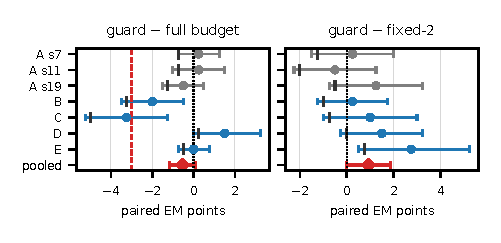
\includegraphics[width=\columnwidth]{figures/fig_samples_main.pdf}
  \caption{Guarded FBG minus full search or two fixed searches. Grey rows rerun
  HotpotQA sample A with new seeds, and blue rows are new question samples.}
  \label{fig:samples}
  \Description{Forest plot of paired exact-match differences between guarded
  FBG and full search or two fixed searches. Each row is one run. Bars show 95 percent
  intervals, ticks show one-sided lower bounds, and a dashed line marks the
  negative three point margin.}
\end{figure}

Figure~\ref{fig:samples} separates decoding and population variation. With the
same 400 questions, decoding seeds 7, 11, and 19 give guarded differences of
$+0.25$, $+0.25$, and $-0.50$ EM. All pass the predeclared rule. Four new
question draws give $-2.00$, $-3.25$, $+1.50$, and $0.00$ EM. Their one-sided
lower bounds are $-3.25$, $-5.00$, $+0.25$, and $-0.50$, so two of four pass
and two fail. Across all five question samples, three of five pass. The two
negative cellwise intervals do not remain directional under the max-t
family-wise band. The draw disagreement is the substantive result because it
overturns the stable decision suggested by same-question decoding reruns.

The draw-level mean is $-0.70$ EM with one-sided lower bound $-2.51$. Pooled
contrasts against full search and fixed-3 are $-0.54$ $[-1.18,0.11]$ and
$-0.32$ $[-1.03,0.37]$ EM, and both contain zero. Contrasts favoring the guard over fixed-2 or repetition use
1.67 and 0.90 more calls. Thus every favorable pooled contrast costs more,
while every equal-cost or lower-cost contrast remains unresolved.

Between-draw contrast variation is larger than the same-question decoding
variation in this small panel. With five question draws and three decoding
seeds, we do not estimate a stable variance decomposition. Descriptively,
$I^2=80\%$ is the share of observed heterogeneity beyond within-draw
uncertainty, while $\tau=1.25$ EM is the estimated between-draw standard
deviation. Neither is a population parameter in this five-draw panel. Only 44
of 2{,}000 questions produce different full-budget and guarded answers, so a
small item set can determine a draw-level decision.

\paragraph{Backbone crosses and Wikipedia-derived datasets.}
Three Claude Haiku 4.5 draws with $n=200$ and one Llama-3.2-3B draw with
$n=400$ all pass the 3-EM margin. Guarded FBG reaches the pooled frontier in
none, and its mean equal-call difference is $+0.14$ EM. Changing the backbone
therefore changes the accuracy level more than the deployment verdict.

On the 25{,}247{,}888-sentence FEVER Wikipedia index, guarded FBG has paired
difference $-0.25$ EM with interval $[-2.00,1.25]$ and lowers calls from 9.00
to 5.90. Fixed-2 still dominates it. Three 2Wiki draws lower calls to between
5.5 and 5.7, but fixed-2 dominates the guard in every draw. On three MuSiQue
draws, answer repetition or fixed-2 also dominates the guard. The repeated
domination extends the result beyond one Wikipedia-derived benchmark. We
interpret these cells as related environments because they share a sparse
retrieval stack and multi-hop task design.

\paragraph{One external news-corpus cell.}
We froze one MultiHopRAG inference-query cell before fitting or test
evaluation. It contains 400 questions over 609 English news articles and uses
Qwen2.5-3B with the same four-search cap. Table~\ref{tab:external-policies}
separates the frozen FBG endpoint from three exploratory signal policies. Each
gain compares a policy to the randomized simple hull at equal
mean calls.

\begin{table}[H]
\caption{External news-cell policies at equal calls to the simple-policy hull.}
\label{tab:external-policies}
\footnotesize
\setlength{\tabcolsep}{8.4pt}
\rowcolors{2}{rowshade}{}
\begin{tabular}{@{}lrrrl@{}}
\toprule
\hiderowcolors
\tabhead \textbf{Policy} & \textbf{EM} & \textbf{Calls} & \textbf{Gain vs.\ simple} & \textbf{95\% CI} \\
\midrule
\showrowcolors
FBG-only & 73.00 & 7.27 & $+0.48$ & $[-0.50,1.46]$ \\
Guarded FBG & 73.25 & 7.40 & $+0.71$ & $[-0.07,1.57]$ \\
Stop classifier & 70.50 & 4.35 & $+2.10$ & $[0.12,4.10]$ \\
Error-head gate & 73.75 & 7.65 & $+1.18$ & $[0.41,2.06]$ \\

\bottomrule
\end{tabular}
\end{table}

Guarded FBG reaches 73.25 EM at 7.40 calls, compared with 72.75 EM at 9.00
calls for full search. It passes the declared endpoint, but the
matched-cost advantage remains unresolved. The binary future-improvement and
error-head intervals are positive, yet both policies are exploratory and come
from one question draw.
The cell therefore shows that the signal choice can change a boundary result.
As a single draw with a per-cell refitted head, it does not establish
cross-domain controller transfer.


\subsection{RQ3: Which stopping signal is informative?}

\paragraph{Current error provides the stronger risk ordering.}
At each selected stop, we rank questions by predicted risk. We define
risk-coverage area as mean stopped-answer error over coverage fractions from
0.05 to 1.00, with lower values preferred, and compare it with 20 random
orderings. We also report expected calibration error (ECE) and area under the
receiver operating characteristic curve (AUROC). Table~\ref{tab:signal-diagnostics}
shows that our current-error head improves on random in every cell, while FBG
does so in 7 of 18. This ordering gap explains how FBG can save calls without
assigning extra search to the questions that benefit from it.

\begin{table}[t]
\caption{Signal and trajectory diagnostics for RQ3. Test labels evaluate the
frozen outputs and never select a policy.}
\label{tab:signal-diagnostics}
\footnotesize
\setlength{\tabcolsep}{3pt}
\rowcolors{2}{rowshade}{}
\begin{tabular}{@{}p{0.31\columnwidth}p{0.17\columnwidth}p{0.43\columnwidth}@{}}
\toprule
\hiderowcolors
Diagnostic & Scope & Measured result \\
\midrule
\showrowcolors
FBG risk ordering & 18 cells & Better than random in 7 cells \\
Error-head ordering & 18 cells & Better than random in all 18 cells \\
Error calibration & 18 cells & Test-prefix ECE 0.019 to 0.087, median 0.043 \\
Gold-support coverage & 18 cells & Cross-fitted AUROC 0.652 to 0.946 \\
Late answer reversals & 1{,}220 pairs & 79 harmful and 14 helpful \\
Rerolled futures & 300 stops & Beat logged best in 10.0\%, changed correctness in 5.7\% \\
\bottomrule
\end{tabular}
\end{table}

\paragraph{Predictive discrimination does not guarantee policy utility.}
Our same-feature gold-support classifier separates evidence-coverage states
with AUROC from 0.652 to 0.946, yet its D/F/I tally is 8/8/2 with no cellwise
equal-call win. The future-improvement classifier is dominated in only one
cell, but its three positive intervals disappear under max-t correction.
State discrimination alone therefore does not establish policy utility.

The current-error target asks whether the present answer is wrong, whereas
FBG must predict a useful later reversal from incomplete prefix information.
The former can rank risk without identifying whether another search will
repair it. Threshold choice and population shift then add two further gaps
between ranking and policy value. These mechanisms are consistent with the
observed diagnostics, not a causal decomposition of the oracle gap.
\paragraph{Late retrieval creates headroom that FBG only partly captures.}
Late retrieval produces 79 harmful and 14 helpful reversals, with a 95\% ratio
interval of 3.2 to 11.1 and $p<10^{-3}$. Guarded FBG realizes 24 beneficial
and 32 harmful flips. FBG captures only part of this stopping headroom.

\paragraph{Refitting and rerolling localize the instability.}
Held-out-prefix FBG correlations range from 0.26 to 0.60 and absolute errors
from 0.12 to 0.19. We therefore repeat fitting and both learned and simple
selection in 400 chain-bootstrap resamples per run. This analysis conditions
on logged questions, retrieval, preprocessing, and decoding, so it isolates
fit-and-selection instability.

\begin{figure}[t]
  \centering
  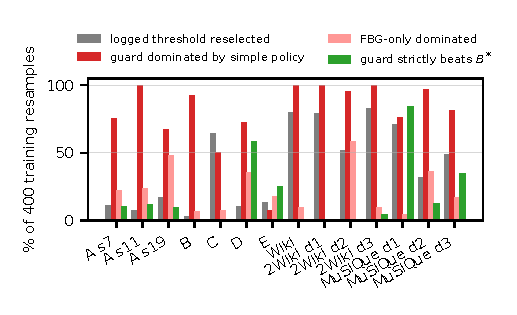
\includegraphics[width=0.88\columnwidth]{figures/fig_nested.pdf}
  \caption{Nested refit and reselection across 400 training-chain resamples per
  fully instrumented run.}
  \label{fig:nested}
  \Description{Grouped bars show the shares of bootstrap replications that
  retain the logged threshold, are dominated by a reselected simple policy,
  or beat the reselected fixed budget.}
\end{figure}

Figure~\ref{fig:nested} makes the selection instability operational. The logged
threshold is reselected in only 3 to 17\% of resamples on six of seven HotpotQA
conditions. A simple policy dominates in 51 to 100\% of resamples in seven of
eight reported runs.

Two rerolled continuations per primary-cell stop beat the logged best in 10.0\%
of cases and change correctness in 5.7\%. These are reachable gains outside the logged path.

The original clipped target variants move mean guarded EM by at most
0.2 points. The logged guarded policies have D/F/I counts 9/3/2 across the
14 instrumented cells. Refitting the full feature set and reselecting the
threshold gives 11/2/1, whereas removing step, evidence-count, and stability
features gives 11/1/2. These are different fitted policies, not conflicting
tallies of the logged matrix: only 8 of 14 refits recover the logged threshold.
Across 154 protocol variants, simple policies dominate 114 and the guard
Pareto-improves $B^\star$ in 17. These probes delimit sensitivity within the
logged regime rather than exclude gains from other designs.

Across 1{,}400 training-size refits, moving from 30 to 90 episodes lowers
domination by 6.1 points and raises mean EM by 0.14, nonmonotonically.
Pooling training chains from same-environment cells (up to 421 episodes) or
all 14 cells (up to 959), excluding target test questions, cuts guarded
domination from 11 to 8 and 9 cells and FBG-only domination from 10 to 4 and 6.
Mean matched-cost gaps remain $-0.22$ to $-0.53$ EM. Of 56 paired intervals,
1 favors the learned policy and 6 the mixture. More data moves points toward
the frontier without resolving a gain (supplement).

\paragraph{Retrospective signed-target and deterministic-control checks.}
On the same 14 cells, a signed best-future target uses the original features,
five-fold training-chain cross-fitting, and threshold grid. The guarded
signed refit has D/F/I counts 11/3/0, compared with 11/2/1 for a freshly
refitted clipped target. Mean EM changes from 22.13 to 22.05, while mean calls
fall from 6.44 to 6.26, isolating clipping, not horizon. We also select a deterministic evidence-growth rule on training chains:
after at least one search, stop when newly retained units are at most a
threshold in $\{0,1,2,3\}$. Adding this rule to the simple family gives
D/F/I counts 11/2/1 for logged guarded FBG and 3/9/2 for FBG-only.
Across calls, tokens, and a wall-time proxy, mean matched-cost gaps are
negative and all 84 conditional simultaneous bands include zero (supplement).
These exploratory checks preserve the frozen 26-cell analysis.
A fresh eight-search Haiku 4.5 check uses 120 training and 200 test questions.
FBG-only reaches 55.5 EM at 8.19 calls, but all 12 conditional simultaneous
matched-cost bands across horizons four and eight include zero (supplement).

\subsection{RQ4: Can we certify stopped answers?}

For each of 14 fully instrumented cells, we reserve 30 of 120 development
episodes, fit the error scorer on 90, and evaluate one guarded-policy stop per
calibration and test episode. Corrected SGR accepts none of the 84 cell and
target-risk pairs over six $\alpha$ values, so Table~\ref{tab:certificate-coverage}
reports zero coverage. This fail-closed result withholds an unsupported
reliability claim.

{\setlength{\intextsep}{6pt}
\begin{table}[t]
\caption{Deployment-matched SGR results for RQ4 with 30 calibration episodes
per cell.}
\label{tab:certificate-coverage}
\footnotesize
\setlength{\tabcolsep}{3pt}
\rowcolors{2}{rowshade}{}
\begin{tabularx}{\columnwidth}{@{}lRRR@{}}
\toprule
\hiderowcolors
\tabhead \textbf{Population} & \textbf{Cells} & \textbf{Accepted pairs} & \textbf{Test coverage} \\
\midrule
\showrowcolors
HotpotQA corpus & 7 & 0/42 & 0\% \\
2WikiMultihopQA & 3 & 0/18 & 0\% \\
MuSiQue & 3 & 0/18 & 0\% \\
Wikipedia 25M & 1 & 0/6 & 0\% \\
\midrule
\hiderowcolors
\textbf{All} & \textbf{14} & \textbf{0/84} & \textbf{0\%} \\
\bottomrule
\end{tabularx}
\end{table}
}

We restrict the claim to deployment-matched prefix features. The supplement
quarantines score-mismatched call-only diagnostics.

